
\documentclass[a4paper,12pt,oneside]{report}

%================ PACKAGES ================
\usepackage{array}
\usepackage{booktabs}
\usepackage{blindtext}
\usepackage{enumitem}
\usepackage{biblatex}
\usepackage{emptypage}
\usepackage[utf8]{inputenc}
\usepackage{graphicx}
\usepackage{glossaries}
\usepackage{dirtytalk}
\usepackage{longtable}
\usepackage{etoolbox}
\usepackage{geometry}
\usepackage{caption}
\usepackage{setspace}
\usepackage{sectsty}
\usepackage{fancyhdr}
\usepackage{tocloft}
\usepackage{tabularx}
\usepackage{float}
\usepackage{multirow}
\usepackage{graphicx}
\usepackage{multirow}
\usepackage{array}
\usepackage{tabularx}
\usepackage{float}
%================ PAGE SETTINGS ================
\renewcommand{\baselinestretch}{1.5}

\geometry{
 a4paper,
 total={170mm,257mm},
 left=1.2in,
 top=1in,
 bottom=1.25in,
 right=1in
}

%================ ORIGINAL FONT SETTINGS ================
% Original LaTeX font retained
% Font size: 12 pt
% Line spacing: 1.5

%================ CHAPTER FORMATTING ================
\chapternumberfont{\vspace{-2cm}\centering\Large\MakeUppercase}
\chaptertitlefont{\vspace{-0.5cm}\centering\Large\MakeUppercase}

\sectionfont{\large\uppercase}
\subsectionfont{\large}

%================ HEADER AND FOOTER ================
\usepackage{fancyhdr}

\setlength{\headheight}{15pt}
\setlength{\headsep}{22pt}

\newcommand{\changefont}{%
\fontsize{10}{12}\selectfont
}

\pagestyle{fancy}
\fancyhf{}

% Chapter name on left only
\fancyhead[L]{\changefont\nouppercase{\thechapter.\leftmark}}

% Page number at centre
\fancyfoot[C]{\thepage}

\renewcommand{\chaptermark}[1]{%
\markboth{#1}{}
}

\renewcommand{\sectionmark}[1]{%
\markright{}
}

\renewcommand{\headrulewidth}{0.5pt}
\renewcommand{\footrulewidth}{0pt}

% Chapter opening pages
\fancypagestyle{plain}{
\fancyhf{}
\fancyhead[L]{\changefont\nouppercase{\leftmark}}
\fancyfoot[C]{\thepage}
\renewcommand{\headrulewidth}{0.5pt}
}

%================ CONTENTS FORMATTING ================
\newcommand{\listequationsname}{List of Equations}

\newlistof{myequations}{equ}{\listequationsname}

\newcommand{\myequations}[1]{%
\addcontentsline{equ}{myequations}
{\protect\numberline{\theequation}#1}\par
}

\renewcommand{\contentsname}{CONTENTS}
\renewcommand{\listfigurename}{LIST OF FIGURES}

\renewcommand{\cfttoctitlefont}
{\hspace*{\fill}\large\bfseries}

\renewcommand{\cftaftertoctitle}
{\hspace*{\fill}}

\renewcommand{\cftlottitlefont}
{\hspace*{\fill}\large\bfseries}

\renewcommand{\cftafterlottitle}
{\hspace*{\fill}}

\renewcommand{\cftloftitlefont}
{\hspace*{\fill}\large\bfseries}

\renewcommand{\cftafterloftitle}
{\hspace*{\fill}}

%================ DOCUMENT ================
\begin{document}

%================ TITLE PAGE ================
\begin{titlepage}
\addtolength{\hoffset}{0cm}
\centering

{\scshape\large\bfseries
AI-Powered Smart Voice Note Maker with Interactive Companion Display\par}

\vspace{0.5cm}

{\scshape\bfseries A COURSE PROJECT REPORT\par}

\vspace{0.3cm}
{\small\bfseries submitted by\par}

\vspace{0.3cm}

{\small\bfseries JOHN PAUL PARET(MUT24CS088)\par}
{\small\bfseries RISHON KUNUKKASSERIL ROSHAN(MUT24CS131)\par}
{\small\bfseries SHREE RASYA G(MUT24CS142)\par}
{\small\bfseries VISHAL V DEVAN(MUT24CS148)\par}

\vspace{0.3cm}
{\small\bfseries as part of the course\par}

\vspace{0.3cm}
{\small\bfseries PBCST504 MICROCONTROLLERS\par}

\vspace{0.3cm}
{\small\bfseries to\par}

\vspace{0.3cm}

{\small\bfseries
The APJ Abdul Kalam Technological University in partial fulfilment of the requirements for the award of the Degree\par}

\vspace{0.3cm}

{\bfseries Bachelor of Technology\par}
{In\par}
{\bfseries Computer Science \& Engineering\par}

\vspace{0.3cm}

\IfFileExists{logo-4.png}{\includegraphics[width=0.50\textwidth]{logo-4.png}}{\fbox{\parbox[c][2cm][c]{0.45\textwidth}{\centering Institute logo placeholder}}}\par

\vspace{0.5cm}

{\bfseries Department of Computer Science \& Engineering\par}
{\bfseries Muthoot Institute of Technology and Science\par}
{\bfseries Kochi - 682308\par}

\vspace{0.5cm}
{\bfseries OCTOBER 2026\par}

\end{titlepage}

%================ CERTIFICATE ================
\begin{titlepage}

\vspace{1.5cm}

\begin{center}
{\scshape\Large\bfseries CERTIFICATE\par}
\end{center}

\vspace{1cm}

\noindent
\textit{This is to certify that the report entitled}
\textbf{``AI-Powered Smart Voice Note Maker with Interactive Companion Display''},
\textit{submitted by}
\textbf{JOHN PAUL PARET
(MUT24CS088), RISHON KUNUKKASSERIL ROSHAN (MUT24CS131), SHREE RASYA G (MUT24CS142), VISHAL V DEVAN (MUT24CS148)}
\textit{to Muthoot Institute of Technology and Science, Kochi for the award of the degree of Bachelor of Technology in Computer Science \& Engineering, is a bonafide record of the course project work carried out by them, as part of the course PBCST504 MICROCONTROLLERS, under my supervision and guidance.}

\vspace{2.5cm}

\noindent
\textbf{Mrs. Sreetha V Kumar}\\
Faculty-in-charge

\vspace{3cm}

\noindent Place: Kochi\\
Date: 02/11/2026

\end{titlepage}

%================ ABSTRACT ================
\newpage
\pagenumbering{roman}
\setcounter{page}{2}
\thispagestyle{plain}

\addcontentsline{toc}{section}{\uppercase\textbf{Abstract}}

\begin{abstract}

The \textbf{AI-Powered Smart Voice Note Maker with Interactive Companion Display} is an intelligent embedded system designed to enhance conventional note-taking through \textbf{real-time voice acquisition}, \textbf{AI-assisted speech processing}, \textbf{wireless communication}, and interactive human--machine interaction. The system employs an \textbf{STM32 microcontroller} for central control, an \textbf{INMP441 digital MEMS microphone} for audio acquisition, an \textbf{ESP32-C3 Wi-Fi module} for network connectivity, and a \textbf{microSD card interface} for persistent data storage. A \textbf{0.96-inch OLED display}, push buttons, an RGB LED, and an active buzzer provide menu navigation, system-status monitoring, and multimodal feedback.

Captured speech is processed through a \textbf{Speech-to-Text (STT) pipeline}, with wireless connectivity enabling interaction with \textbf{external computational services} for advanced language processing and AI-driven functionalities. Potential extensions include \textbf{conversational interaction}, \textbf{automatic summarization}, \textbf{semantic keyword extraction}, and \textbf{intelligent note classification and organization}. The microcontroller coordinates peripheral communication, user input, data management, and interaction between the embedded hardware and external processing infrastructure.

The project demonstrates the integration of \textbf{embedded computing}, \textbf{digital audio acquisition}, \textbf{peripheral interfacing}, \textbf{wireless networking}, \textbf{persistent data management}, and \textbf{artificial intelligence} within an extensible assistive technology platform. By combining \textbf{resource-constrained microcontroller hardware} with externally hosted intelligent processing, the system aims to provide an accessible alternative to manual note-taking, supporting \textbf{context-aware information capture}, \textbf{efficient knowledge retrieval}, and improved productivity for students and professionals.

\end{abstract}

%================ CONTENTS ================
\newpage
\tableofcontents

\newpage
\renewcommand\thepage{\arabic{page}}

\clearpage
\pagenumbering{arabic}
\setcounter{page}{1}

%================ CHAPTER 1 ================
\chapter{INTRODUCTION}


\section{PURPOSE OF THE SYSTEM}


\setlength{\parindent}{0pt}
\setlength{\parskip}{6pt}

\noindent
The purpose of the AI-Powered Smart Voice Note Maker with Interactive Companion Display is to develop a smart and user-friendly system that simplifies the process of capturing, recording, and organizing spoken information. It provides an alternative to conventional note-taking methods by allowing users to record their thoughts, ideas, reminders, and important information through voice-based interaction.

\noindent
The system uses an STM32 microcontroller as its primary control unit, interfaced with an INMP441 digital MEMS microphone for capturing voice input. The ESP32-C3 module provides wireless connectivity for communication with external processing services, while a microSD card interface supports data storage. An OLED display, push buttons, RGB LED, and buzzer provide an interactive interface for user control and system feedback.

\noindent
Through speech-to-text processing and AI-assisted analysis, the system aims to convert spoken information into readable text, identify important details, and organize the generated notes for easy access and retrieval. This helps reduce the effort involved in manual documentation and makes recorded information easier to review and manage.

\noindent
The system is intended for students, educators, and working professionals who frequently need to capture information during lectures, meetings, and discussions. It can also be used for recording personal ideas, reminders, and everyday tasks. Overall, the proposed system aims to provide a compact and convenient note-taking solution by integrating embedded hardware, wireless communication, and AI-assisted information processing.


\section{RELEVANCE AND SCOPE OF THE SYSTEM}


In modern academic and professional environments, the ability to
efficiently capture, organize, and retrieve information is essential.
Students, educators, and working professionals frequently encounter
situations such as lectures, meetings, discussions, and brainstorming
sessions where important information must be recorded accurately.
However, conventional note-taking methods rely heavily on manual
writing or typing, which can divide the user's attention and result
in missed information, incomplete notes, and reduced concentration.

Although digital audio-recording applications provide an alternative
to manual note-taking, they primarily preserve information in the
form of lengthy recordings. Reviewing these recordings to identify
important points, extract key information, and organize content
requires additional time and effort. This highlights the need for
a more intelligent and efficient approach to information management.

The proposed \textit{AI-Powered Smart Voice Note Maker with
Interactive Companion Display} addresses this challenge through
the integration of embedded hardware, voice input, speech-to-text
processing, and AI-assisted information organization. The system
aims to transform spoken information into structured and accessible
notes while providing an interactive interface for user control
and system feedback.

The relevance of the proposed system can be identified in the
following applications:

\begin{itemize}
    \item \textbf{Academic Applications:}
    Enables students to capture important information during
    lectures and discussions, reducing dependence on continuous
    manual note-taking.

    \item \textbf{Professional Applications:}
    Assists in recording and organizing information obtained
    during meetings, interviews, and professional discussions.

    \item \textbf{Personal Productivity:}
    Provides a convenient method for recording ideas, reminders,
    and tasks through voice-based interaction.

    \item \textbf{Accessibility:}
    Offers an alternative method of information capture for
    individuals who experience difficulty or inconvenience
    with conventional methods.
\end{itemize}

%================ CHAPTER 2 ================
\chapter{PROBLEM DEFINITION}

\section{PROBLEM STATEMENT}

Conventional note-taking methods rely on manual writing or typing
to record information during lectures, meetings, and discussions.
This often divides the user's attention between listening and
recording, resulting in missed details and incomplete notes.
Although digital audio-recording applications provide an alternative,
they generally store information as lengthy audio files that require
additional time and effort to review, transcribe, and organize.
Furthermore, extracting key points and identifying important tasks
from recorded information can be challenging. Therefore, there is
a need for an intelligent and compact system that can acquire
spoken information, convert audio into text, and facilitate the
organization and retrieval of important content. The proposed
\textit{AI-Powered Smart Voice Note Maker with Interactive
Companion Display} addresses this need by integrating an STM32-based
embedded control system, digital audio acquisition, speech-to-text
processing, wireless communication, and AI-assisted information
organization to provide an efficient and interactive note-taking
solution.

\section{OBJECTIVES}

The primary objectives of the proposed system are:

\begin{enumerate}
    \item To design and develop a compact and portable smart
    voice note-taking device using the STM32 microcontroller
    as the central processing and control unit.

    \item To acquire spoken information using a digital MEMS
    microphone and interface it with the microcontroller
    through an appropriate digital audio communication protocol.

    \item To implement audio capture and processing mechanisms
    that enable the conversion of spoken input into text
    using speech-to-text technology.

    \item To incorporate AI-assisted processing for extracting
    key information, identifying important tasks, and organizing
    transcribed content into meaningful notes.

    \item To integrate an OLED display and push-button controls
    for providing a user-friendly interface and enabling
    interactive operation of the device.

    \item To implement suitable data storage and wireless
    communication interfaces for managing recorded information
    and facilitating communication with external processing
    services.

    \item To incorporate visual and audible feedback mechanisms
    using an RGB LED and buzzer to indicate system status,
    user inputs, and important notifications.
\end{enumerate}



%================ CHAPTER 3 ================
% Requires: booktabs, tabularx. Include inside an existing report document.
\chapter{Requirement Analysis}
\label{ch:requirements}

The proposed smart voice note maker combines an STM32-based audio and display unit with an ESP32 network interface and a server-hosted note management application. Speech is captured as digital audio and transferred to the server; transcription and structured note generation are requested separately through the web interface. The requirements below describe the STM32--ESP32 firmware configuration present in the repository. The repository also retains an earlier ESP32-only implementation.

\section{Hardware Components Required}
Table~\ref{tab:hardware} identifies the components required by the split implementation. Board quantities, exact module variants and the final power arrangement should be confirmed against the physical prototype.
\begin{table}[htbp]
\centering
\caption{Hardware requirements for the STM32--ESP32 configuration}
\label{tab:hardware}
\small
\begin{tabularx}{\textwidth}{@{}lX X@{}}
\toprule
Component & Configuration in project materials & Role \\
\midrule
STM32 board & Nucleo-F446RE; PlatformIO \texttt{nucleo\_f446re} target & I2S audio capture, UART transfer and OLED control. \\
ESP32 board & PlatformIO \texttt{esp32dev} target; physical board variant to be verified & Wi-Fi, server polling and HTTP audio upload. \\
Microphone & INMP441 digital I2S microphone, left channel selected & Converts speech to serial digital audio. \\
Display & SSD1306 I2C OLED, 128 $\times$ 64 pixels, address \texttt{0x3C} & Displays text describing recording and connection status. \\
Power and interconnections & Separate USB power for the two boards; common ground; connecting leads & Supplies power and carries I2S, I2C and UART signals. Exact construction to be verified. \\
Host and network & Server host and Wi-Fi/LAN accessible to the device and web client & Runs the application, stores recordings and presents the browser interface. \\
\bottomrule
\end{tabularx}
\end{table}

\textbf{STM32 Nucleo-F446RE:} The controller acquires microphone data, transfers audio blocks and updates the local display.

\textbf{INMP441 microphone:} The digital microphone provides the serial audio input. Its channel-selection connection determines the slot used by the capture code.

\textbf{ESP32:} The network controller connects to Wi-Fi, retrieves recording commands and uploads the WAV stream to the server.

\textbf{SSD1306 display:} The OLED presents brief messages for the local user, including recording and upload status.

The microphone and display are assigned to the STM32. The STM32 uses I2S2 with direct memory access (DMA) for acquisition, I2C for the display and USART6 for the ESP32 link. The ESP32 provides connectivity to the server. The display code renders text and a separator line; animated facial expressions are not implemented in this split firmware. Compatibility of the particular OLED module with a 3.3~V supply and the availability of ESP32 GPIO16 and GPIO17 must be checked.

\section{Software/Firmware Tools Used}
\begin{table}[htbp]
\centering
\caption{Software and configuration requirements}
\label{tab:software}
\small
\begin{tabularx}{\textwidth}{@{}lX@{}}
\toprule
Software & Purpose and configuration \\
\midrule
PlatformIO and Arduino framework & Separate \texttt{ststm32} and \texttt{espressif32} firmware projects; STM32 code also uses the HAL for I2S and DMA. \\
Display libraries & Adafruit SSD1306 and Adafruit GFX in the STM32 project. \\
ArduinoJson & Parses server responses in the ESP32 project. \\
Python server & FastAPI, Uvicorn, SQLAlchemy, Jinja2 and other dependencies listed in \texttt{server/requirements.txt}. \\
Storage & SQLite by default, with audio files stored on disk; a PostgreSQL configuration is also provided. \\
AI service & Gemini through the server's Google Gen AI client; an API key is required for AI processing, but not for audio-only recording. \\
Browser and network & Authenticated web interface for recording requests, playback and optional AI processing; device API key for device endpoints. \\
\bottomrule
\end{tabularx}
\end{table}

The ESP32 requires a private \texttt{secrets.h} containing Wi-Fi credentials, a server origin and the matching device API key. Server settings include the device key, session secret, administrator credentials, audio storage and optional Gemini configuration. The split client accepts a plain HTTP origin without a path. The API uses an API key, but plain HTTP does not encrypt the key or audio; the supplied documentation therefore confines this setup to a trusted local network or a protected connection.

The general software sequence is as follows:
\begin{enumerate}
\item Initialize the controller interfaces and establish Wi-Fi connectivity.
\item Receive a recording request through the server.
\item Acquire audio on the STM32 and transfer it to the ESP32.
\item Stream the WAV recording to the server and display the returned status.
\item Store the recording for playback and, when requested, generate an AI note.
\end{enumerate}

\section{Feasibility Analysis}
\subsection{Technical Feasibility}
The implemented separation assigns audio capture and local display control to the STM32 and network operations to the ESP32. At 16~kHz, 16-bit mono, the audio payload rate is $16{,}000\times 2=32{,}000$ bytes/s. A 60~s recording therefore contains approximately 1.92~MB of PCM data, excluding the WAV header and transfer overhead. Streaming blocks through UART and chunked HTTP avoids keeping the entire recording in microcontroller memory. At the configured 921600~baud the nominal serial capacity is sufficient for this payload rate, subject to framing, processing and buffering. The implementation detects several transfer failures.

The server, rather than the STM32, invokes Gemini when requested by the user. The STM32F446RE is not used to run a local Whisper model; the computationally intensive AI operation is assigned to the server and external service. Feasibility of AI processing consequently depends on the server configuration, service availability and network access.

\subsection{Operational Feasibility}
The web interface provides a record request, playback and an explicit AI-generation action. The local OLED reports brief text states. This workflow requires the device, server and network to be available; the split firmware provides neither offline recording nor automatic retry of an already delivered command. The current firmware does not initiate voice-question requests, although the server exposes an \texttt{/api/ask} endpoint.

\subsection{Economic and Implementation Feasibility}
The design uses development boards and existing software libraries, with a host computer providing storage and AI integration. No verified bill of materials, component prices, service charges or prototype expenditure is supplied; a quantitative cost analysis remains to be completed. The separate firmware projects support modular development and integration of the controller and network functions.

%================ CHAPTER 4 ================
\chapter{SYSTEM DESIGN}

This chapter describes the functional architecture, circuit interconnections, component arrangement and working sequence of the smart voice note maker. The STM32 handles audio acquisition and the local display, while the ESP32 provides the network connection to the server and web interface.

\section{BLOCK DIAGRAM OF THE HARDWARE SYSTEM}
Figure~\ref{fig:hardware_block_diagram} illustrates the relationship between the microphone, the two controllers, the display and the server. The user requests a recording through the web interface; the STM32 captures the microphone input and the ESP32 streams it to the server. The server stores the recording and can request AI processing when selected by the user.

\begin{figure}[htbp]
\centering
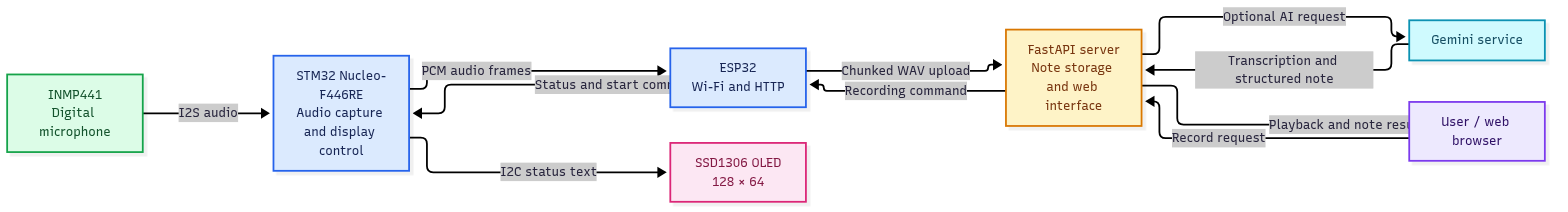
\includegraphics[width=\textwidth,height=0.55\textheight,keepaspectratio]{figures/system_architecture.png}
\caption{Functional block diagram of the smart voice note maker.}
\label{fig:hardware_block_diagram}
\end{figure}

The main functional blocks are described below:
\begin{enumerate}
\item \textbf{Voice input and microphone:} The INMP441 captures spoken information and supplies digital audio over I2S.
\item \textbf{STM32 Nucleo-F446RE:} The controller receives audio using I2S and DMA, communicates with the ESP32 over UART and drives the OLED display.
\item \textbf{ESP32 network controller:} The ESP32 connects to Wi-Fi, polls for recording requests and streams the audio to the server over HTTP.
\item \textbf{OLED display:} The SSD1306 display presents brief text messages for connection, recording and upload status.
\item \textbf{Server and web interface:} The server stores the recording and presents it for playback. The user can request transcription and structured note generation through the web interface.
\item \textbf{AI service:} When requested, the server submits the audio to Gemini and stores the generated transcript and note fields.
\end{enumerate}

\section{CIRCUIT SCHEMATIC / WIRING DIAGRAMS}
The INMP441 microphone and SSD1306 display are connected to the STM32 through I2S and I2C, respectively. The ESP32 exchanges audio and control frames with the STM32 over a crossed UART connection. Both boards share a common ground and use separate USB power. Figure~\ref{fig:circuit_schematic} shows the firmware-defined signal connections; it is a logical wiring diagram rather than a PCB schematic. The individual pin assignments are listed in Table~\ref{tab:wiring}.

\begin{figure}[htbp]
\centering
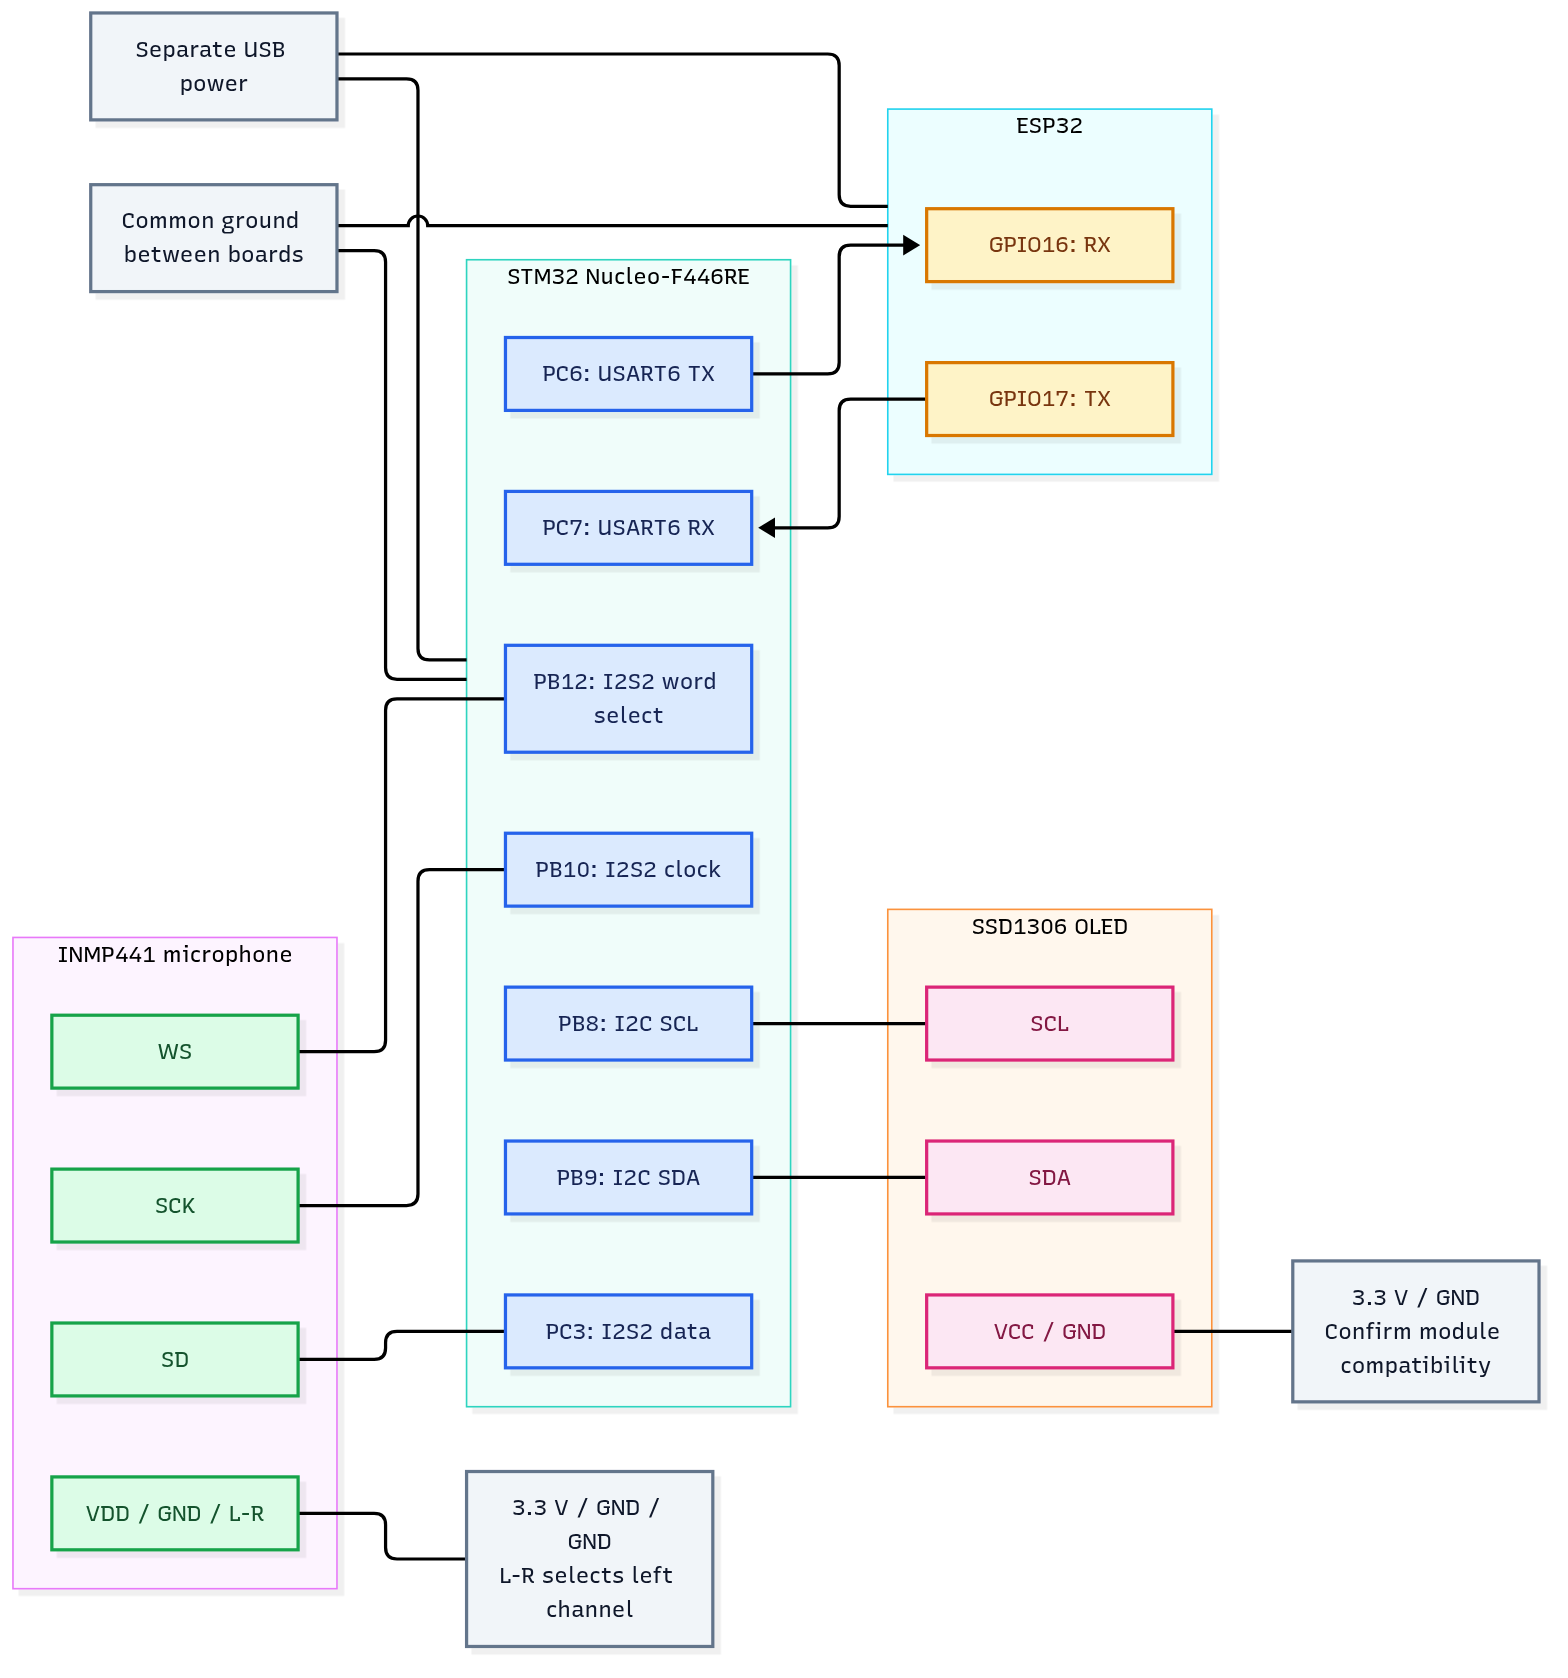
\includegraphics[width=\textwidth,height=0.70\textheight,keepaspectratio]{figures/wiring.png}
\caption{Logical wiring diagram for the STM32--ESP32 configuration.}
\label{fig:circuit_schematic}
\end{figure}

% Figures are supplied as PNG files in the figures directory.

\section{Component Layout / PCB Design}
\label{sec:layout}
The available project materials describe a development-board interconnection, rather than a verified custom printed circuit board. The intended functional arrangement places the INMP441 microphone and SSD1306 display on the STM32 side and connects the ESP32 as the network interface. Figure~\ref{fig:layout} reserves space for a photograph or drawing of the physical component layout.
\begin{figure}[htbp]
\centering
\fbox{\parbox[c][50mm][c]{0.82\textwidth}{\centering Component layout photograph or drawing\\[2mm] (to be supplied)}}
\caption{Physical layout of the hardware components (placeholder).}
\label{fig:layout}
\end{figure}

The signal allocation in Table~\ref{tab:wiring} follows the STM32 and ESP32 firmware. The functional arrangement is presented independently of a physical PCB layout; a board drawing should be supplied if a custom PCB is used.
\begin{table}[htbp]
\centering
\caption{Firmware-defined interconnections for the split design}
\label{tab:wiring}
\small
\begin{tabularx}{\textwidth}{@{}l l X@{}}
\toprule
Module signal & Connection & Function \\
\midrule
INMP441 SCK & STM32 PB10 & I2S2 clock \\
INMP441 WS & STM32 PB12 & I2S2 word select \\
INMP441 SD & STM32 PC3 & I2S2 serial data input \\
INMP441 VDD, GND, L/R & 3.3~V, GND, GND & Supply, ground and left-channel selection \\
OLED SDA, SCL & STM32 PB9, PB8 & I2C data and clock \\
OLED VCC, GND & 3.3~V, GND & Supply; verify module compatibility \\
STM32 PC6 TX & ESP32 GPIO16 RX & STM32-to-ESP32 UART \\
STM32 PC7 RX & ESP32 GPIO17 TX & ESP32-to-STM32 UART \\
Board grounds & Common GND & Shared signal reference \\
\bottomrule
\end{tabularx}
\end{table}

The following layout considerations guide the integration of the modules:
\begin{itemize}
\item Keep the microphone accessible to the speaker and the display visible to the user.
\item Identify the microphone, display and UART connections clearly to simplify inspection and maintenance.
\item Maintain a common ground between the controllers and check supply polarity and module voltage compatibility.
\item Arrange the leads so that the microphone and communication connections remain secure during operation.
\item Preserve access to the USB connections used for programming, power and serial monitoring.
\end{itemize}

\section{Working Principle and Flowcharts}
\label{sec:working}
\subsection{Recording and Transfer}
The STM32 initializes its serial link at 921600~baud and attempts to initialize the OLED. The ESP32 periodically connects to Wi-Fi as needed and polls the server for a pending record command at a nominal five-second interval. A user initiates this command through the web interface. Once a command is received, the ESP32 opens an HTTP connection, sends a WAV header using chunked transfer encoding and sends a \texttt{START} frame containing the recording duration to the STM32.

The STM32 starts I2S2 in master receive mode at 16~kHz with 32-bit slots and circular DMA. It discards 40 startup blocks of 128 samples before sending \texttt{HELLO}. During capture, DMA callbacks place 128-sample blocks in a bounded queue; the code takes the most significant 16 bits of the selected left slot and sends little-endian PCM in numbered \texttt{AUDIO} frames. The ESP32 checks frame sequence and length and sends the received payload as HTTP chunks. After the expected samples, the STM32 sends \texttt{END}; the ESP32 checks its sequence, terminates the HTTP stream and reads the server response. Initialization failure, queue overrun, invalid or missing frames, timeout or network write failure can terminate the transfer. The OLED receives short status messages; the split ESP32 code does not poll the note status endpoint after upload.

\begin{figure}[htbp]
\centering
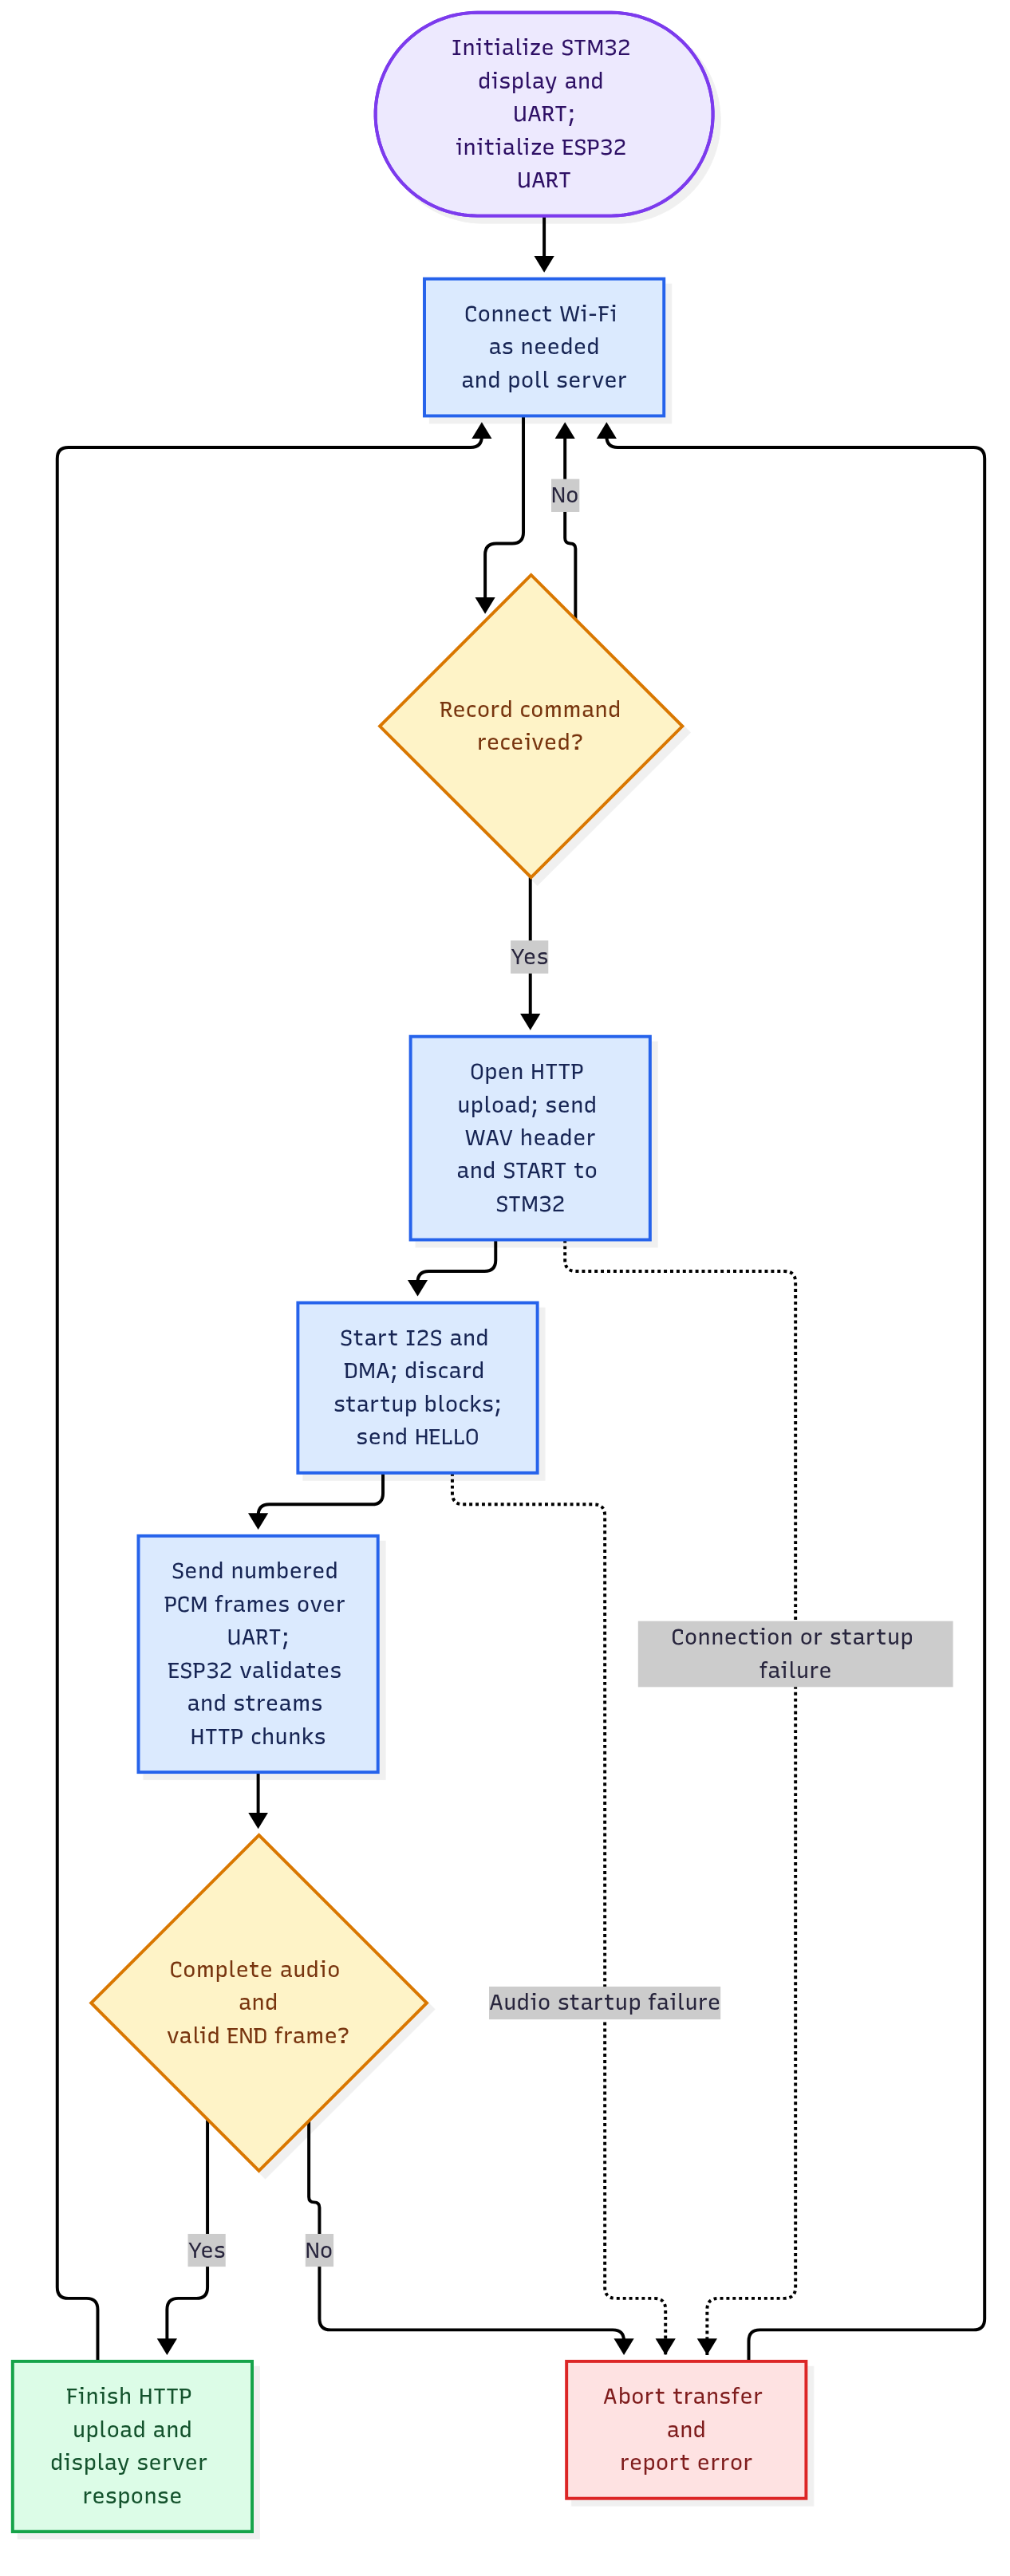
\includegraphics[width=\textwidth,height=0.68\textheight,keepaspectratio]{figures/recording_flow.png}
\caption{Principal recording and upload flow of the STM32--ESP32 firmware.}
\label{fig:record-flow}
\end{figure}

The principal sequence can be summarized as follows:
\begin{enumerate}
\item Initialize the display and serial interfaces and connect the ESP32 to Wi-Fi.
\item Poll for a record command created through the web interface.
\item Open the upload, send the WAV header and request STM32 capture.
\item Initialize I2S and DMA, discard startup samples and acknowledge readiness.
\item Transfer numbered audio blocks to the ESP32 and stream them to the server.
\item Check the end frame and server response, then display the resulting status.
\item Return to command polling; report and abort the transfer if a capture or communication error occurs.
\end{enumerate}

\subsection{Server Storage and Optional AI Processing}
The server authenticates the device, validates the WAV format and stores the audio and note metadata. A successful upload creates a \texttt{recorded} note and completes the associated command. The user may play the recording immediately. AI processing starts only when requested from the website; the server then submits the audio to Gemini for transcription and structured fields such as title, summary, key points, tasks and tags. Failed processing retains the recording for a later retry. The companion OLED reports the immediate upload response in the split implementation, while the web interface presents the AI results.
\begin{figure}[htbp]
\centering
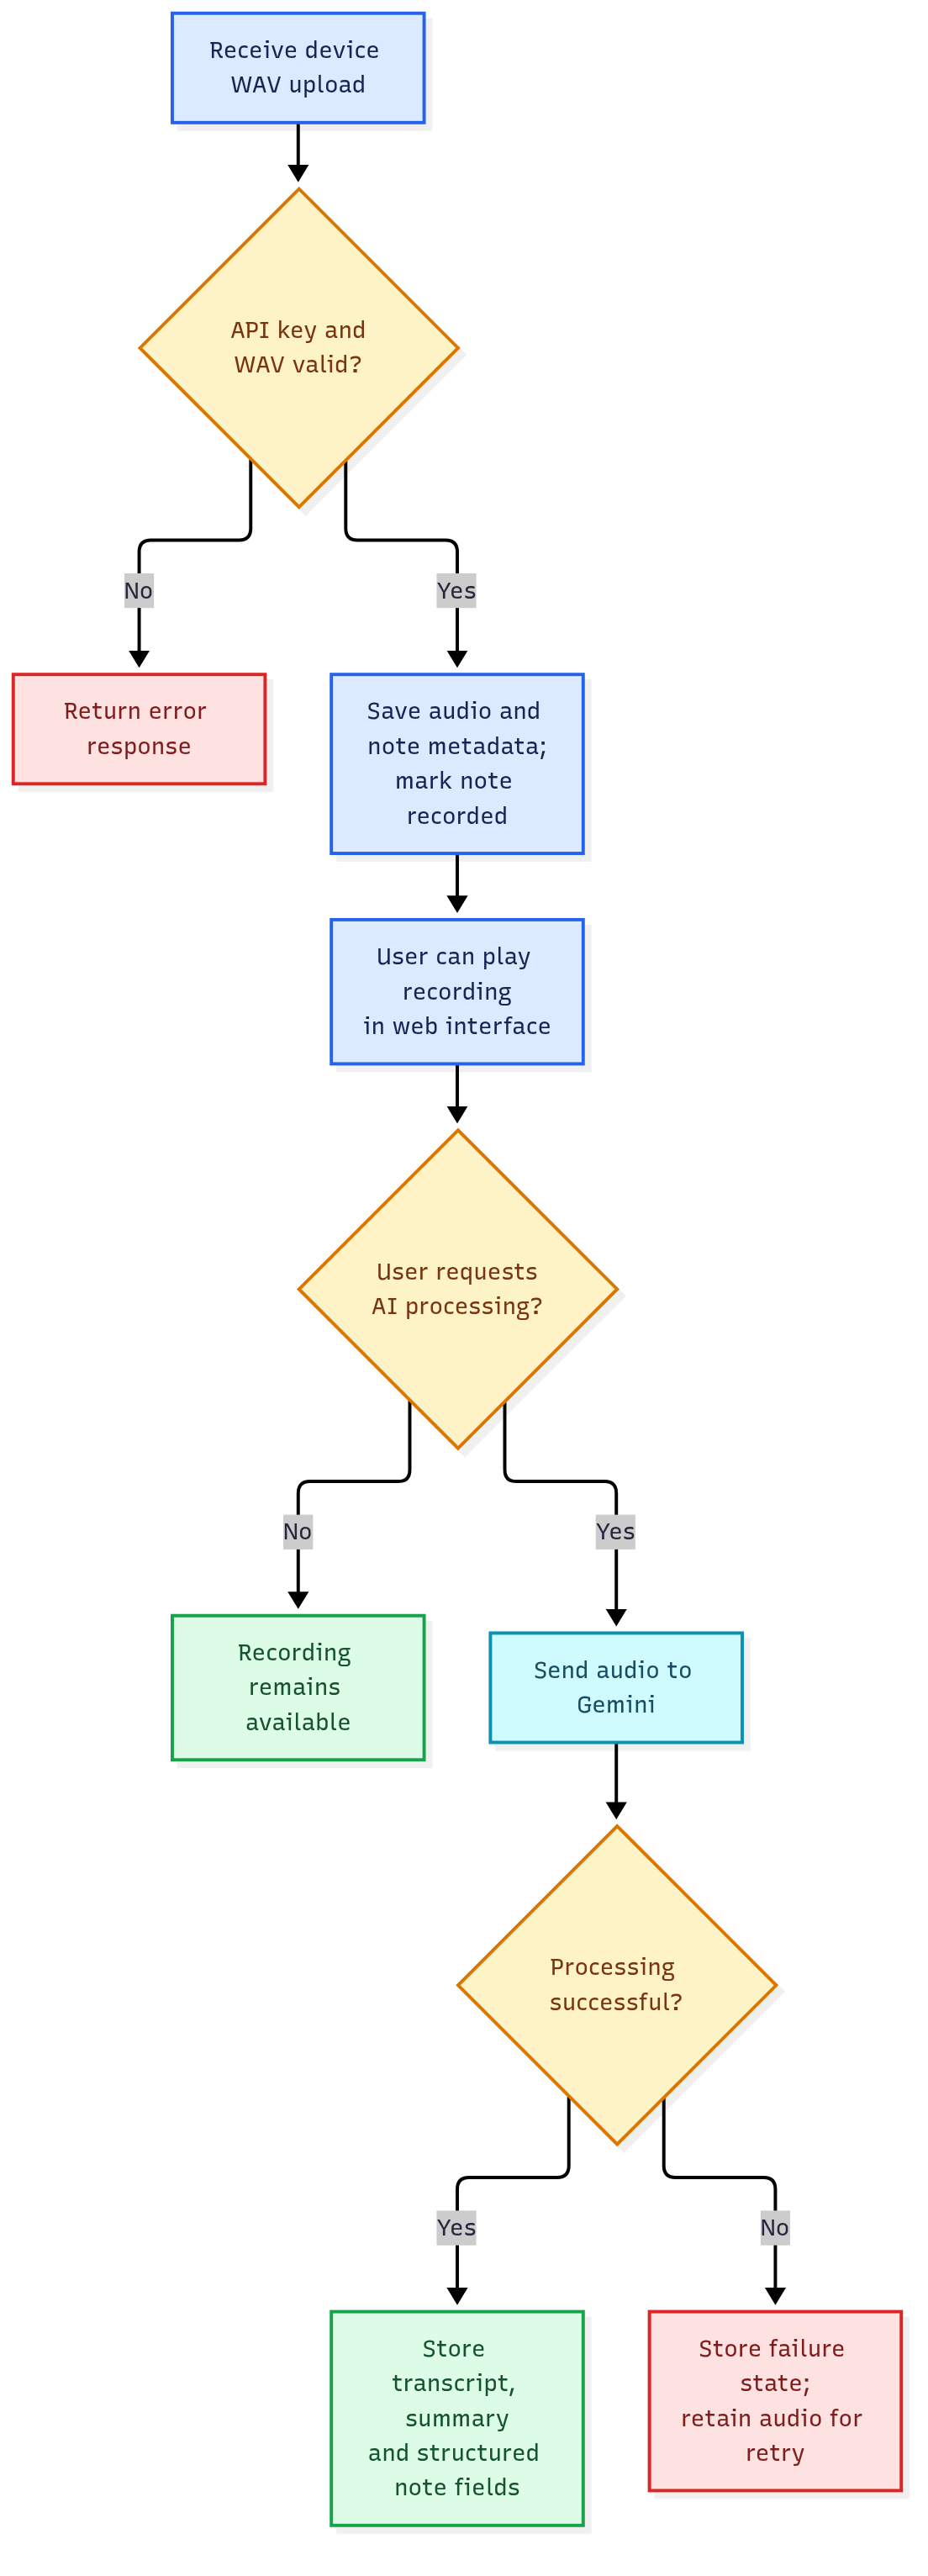
\includegraphics[width=\textwidth,height=0.62\textheight,keepaspectratio]{figures/server_processing.png}
\caption{Server-side note storage and optional AI processing.}
\label{fig:server-flow}
\end{figure}

%================ CHAPTER 5 ================
% Requires: booktabs, tabularx, graphicx.
\chapter{Implementation}
\label{ch:implementation}

This chapter presents the integration of the audio acquisition, display, network and server components of the smart voice note maker. The assembly procedure is based on the firmware-defined connections and the current project wiring documentation.

\section{Step-by-Step Assembly of the Hardware Prototype}
The arrangement uses an STM32 Nucleo-F446RE as the audio and display controller and an ESP32 as the Wi-Fi interface. The INMP441 and OLED are connected to the STM32, while the two controllers exchange commands, audio and status over UART. Each board is intended to receive power through its own USB connection, with a common ground between them. The interconnections are listed in Table~\ref{tab:wiring}.

The hardware integration procedure follows these steps:
\begin{enumerate}
\item Identify the power, ground and signal pins on both development boards and modules.
\item Connect the INMP441 microphone supply, channel selection and I2S signals to the STM32.
\item Connect the SSD1306 supply and I2C signals to the STM32.
\item Cross-connect the STM32 and ESP32 UART transmit and receive signals and establish a common ground.
\item Inspect supply polarity, signal connections and board pin availability.
\item Connect separate USB power to the two boards and program each controller with its respective firmware.
\end{enumerate}

\section{Circuit Integration and Wiring Details}
\subsection{Microphone and Display Connections}
Connect the microphone SCK, WS and SD signals to PB10, PB12 and PC3, respectively. Connect its VDD to 3.3~V, its ground to the common ground and its L/R input to ground for left-channel operation. The project documentation calls for checking the microphone breakout for the recommended 100~k$\Omega$ SD pull-down before adding one. Connect OLED SDA and SCL to PB9 and PB8 and connect its supply and ground after confirming that the module supports 3.3~V. The firmware initializes the display at I2C address \texttt{0x3C}.

\subsection{Controller Interconnection and Power}
Connect STM32 PC6 (transmit) to ESP32 GPIO16 (receive), and ESP32 GPIO17 (transmit) to STM32 PC7 (receive). Connect the grounds together and power the boards independently by USB as specified in the current wiring documentation. Confirm the availability of the ESP32 pins on the actual board and check the wiring and supply polarity before energizing the assembly. The pin assignments follow the current firmware configuration.

\section{Firmware/Code Flashing and Configuration}
\subsection{Build and Configuration}
The STM32 and ESP32 are separate PlatformIO projects in \texttt{firmware/stm32} and \texttt{firmware/esp32}. The former targets \texttt{nucleo\_f446re} and the latter \texttt{esp32dev}, both using the Arduino framework. The STM32 project includes the Adafruit display libraries, and the ESP32 project uses ArduinoJson. The STM32 code additionally configures the I2S and DMA peripherals through the HAL.

For the network client, copy \texttt{firmware/esp32/include/secrets.example.h} to \texttt{secrets.h} in the same directory and configure Wi-Fi, the plain HTTP server origin and the device API key. Configure the server from \texttt{server/.env.example}, including matching device credentials, a session secret, an administrator password and, if AI processing is required, a Gemini API key. Credentials should remain outside the report and version control. The following commands build and upload the two projects independently from the repository root:
\begin{verbatim}
pio run -d firmware/stm32
pio run -d firmware/stm32 -t upload
pio run -d firmware/esp32
pio run -d firmware/esp32 -t upload
\end{verbatim}
The server dependencies are listed in \texttt{server/requirements.txt}; the server is started using \texttt{python run.py} from the \texttt{server} directory after its environment is configured. The default firmware duration is 60~s. If changed, the server's maximum audio duration and command lifetime must be sufficient for the chosen recording and upload.

\subsection{STM32 Audio and Display Firmware}
The STM32 configures SPI2 as an I2S master receiver, using DMA1 stream~3 in circular mode. DMA callbacks copy the selected left-channel data into a 16-entry ring of 128-sample blocks. The foreground code converts each block to a framed 16-bit PCM payload and transmits it over USART6. A full queue or I2S error sets an overflow condition and stops the recording. Display routines initialize the 128~$\times$~64 OLED over I2C and render a title and message. If display initialization fails, messages continue to be sent to the USB serial log; the display is not assumed to be operational.

\subsection{ESP32 Network and Link Firmware}
The ESP32 polls the device-command endpoint, initiates the upload and forwards the server response to the STM32 as a status message. Its UART receive buffer is configured to 32768 bytes. The shared binary protocol uses a two-byte marker, version, type, sequence number, bounded payload length and CRC-16/CCITT-FALSE. The receiver discards malformed frames and the upload path checks audio sequence, size and the final \texttt{END} frame. The ESP32 constructs a 44-byte PCM WAV header and streams the audio in HTTP chunks instead of allocating an entire recording buffer.

\subsection{Server and User Interface}
The FastAPI application stores audio on disk and metadata in a database, SQLite by default. The browser interface allows a logged-in user to request a recording and play saved audio. AI generation is a separate user action; its output and failure state are stored with the note. An optional question-answering endpoint is present on the server, but the split firmware does not call it. Likewise, the older ESP32-only firmware in \texttt{firmware/voice\_note} is a separate implementation and should not be mixed with the split wiring described here.

\section{Challenges and Design Responses}
The following engineering constraints and responses are evidenced by the source and project documentation. They describe design considerations and the corresponding implementation choices.
\begin{enumerate}
\item \textbf{Continuous audio transfer:} A minute of uncompressed PCM occupies approximately 1.92~MB. The design uses DMA blocks, UART frames and chunked HTTP streaming to avoid storing the entire recording on either controller.
\item \textbf{Transfer integrity and buffering:} The finite capture queue can overflow and the serial or network link can lose or delay data. Sequence numbers, CRC checking, timeouts and abort messages allow the firmware to reject incomplete transfers.
\item \textbf{Microphone startup:} The STM32 discards 40 initial audio blocks before signalling readiness, as implemented in the recording routine.
\item \textbf{Pin allocation:} The microphone, display and inter-controller link each require distinct peripheral signals. The design assigns I2S2, I2C and USART6 to separate pins, as listed in Table~\ref{tab:wiring}.
\item \textbf{AI and network dependence:} The STM32 does not run the transcription model. Optional AI generation requires the configured server and external Gemini service; upload also depends on network connectivity. The split firmware does not provide offline recording or automatic retry of a delivered command.
\end{enumerate}

\section{Photographs of the Hardware Model}
The following placeholders should be replaced with actual project photographs after checking that they show the stated configuration.
\begin{figure}[htbp]
\centering
\fbox{\parbox[c][45mm][c]{0.8\textwidth}{\centering Photograph placeholder: overall STM32--ESP32 assembly}}
\caption{Overall assembly of the voice note maker (photograph to be supplied and verified).}
\label{fig:assembly-photo}
\end{figure}
\begin{figure}[htbp]
\centering
\fbox{\parbox[c][45mm][c]{0.8\textwidth}{\centering Photograph placeholder: microphone, OLED and controller wiring}}
\caption{Microphone, display and inter-controller wiring (photograph to be supplied and verified).}
\label{fig:wiring-photo}
\end{figure}
\begin{figure}[htbp]
\centering
\fbox{\parbox[c][45mm][c]{0.8\textwidth}{\centering Screenshot placeholder: recorded note and optional AI output}}
\caption{Web interface showing a recorded note and its AI output (screenshot to be supplied and verified).}
\label{fig:web-photo}
\end{figure}



%================ CHAPTER 6 ================
\newpage
\chapter{TESTING, RESULTS, AND PERFORMANCE ANALYSIS}

\section{TESTING PROCEDURES}


Testing is carried out to verify the proper functioning, reliability,
and integration of the hardware and software components of the
proposed system. Each module is initially tested independently,
followed by integrated testing to ensure that all components
operate together as intended.

\begin{enumerate}

    \item \textbf{Power Supply Testing:}

    The power supply connections are inspected, and the output
    voltages are measured using a digital multimeter. The voltage
    levels are verified against the operating requirements of
    the STM32 microcontroller and connected peripheral modules.
    This test ensures stable power delivery and prevents
    improper operation due to voltage fluctuations.

    \item \textbf{Microcontroller Testing:}

    The STM32 microcontroller is programmed with a basic test
    firmware to verify successful initialization and execution.
    GPIO operations and peripheral communication interfaces
    are checked to ensure that the controller responds correctly
    to input signals and executes the programmed instructions.

    \item \textbf{Microphone Testing:}

    The INMP441 digital MEMS microphone is tested by capturing
    audio samples through the I\textsuperscript{2}S interface.
    Different sound levels and speech inputs are provided to
    verify audio acquisition and signal reception. The captured
    samples are examined to identify noise or signal interruptions.

    \item \textbf{OLED Display Testing:}

    The SSD1306 OLED display is tested by initializing the
    I\textsuperscript{2}C communication interface and displaying
    sample text and system-status messages. The display is
    checked for proper initialization, readability, and
    correct updating of information.

    \item \textbf{User Input and Feedback Testing:}

    The push buttons are tested individually to verify correct
    detection of user inputs. The RGB LED and buzzer are also
    tested to confirm proper visual and audible indications
    during different system operations.

    \item \textbf{Wireless Communication Testing:}

    The ESP32-C3 module is tested for wireless network
    connectivity and communication with the intended external
    processing service. Successful data transmission and
    reception are verified under available network conditions.

    \item \textbf{Integrated System Testing:}

    All hardware and software modules are integrated and tested
    together. Voice input is captured, processed through the
    implemented speech-to-text workflow, and converted into
    text-based notes. The storage, display, and user interaction
    functions are also verified to ensure coordinated system
    operation.

    \item \textbf{Calibration and Performance Testing:}

    The microphone response is evaluated at different
    speaking distances and sound levels. Audio quality,
    transcription accuracy, processing time, storage reliability,
    and system response are observed. Necessary adjustments
    are made to improve the overall performance and reliability
    of the prototype.

\end{enumerate}

\vspace{3cm}


\section{ACTUAL SYSTEM READINGS, OUTPUT DATA, AND PERFORMANCE GRAPHS}

%================ CHAPTER 7 ================
\newpage
\chapter{COST ESTIMATION AND FINANCIAL ANALYSIS}
The total project expenditure is evaluated to understand its affordability and feasibility. A comparison with conventional voice recorders and commercial AI-powered note-taking solutions is also provided to highlight the features, advantages, and cost-effectiveness of the proposed system.

\section{BILL OF MATERIALS (BOM) WITH COMPONENT PRICES}



\section{TOTAL DEVELOPMENT COST VS. COMMERCIAL ALTERNATIVES}

%================ CHAPTER 8 ================
\chapter{CONCLUSION AND FUTURE SCOPE}

\section{SUMMARY OF ACHIEVEMENTS AND PROJECT IMPACT}

\section{CURRENT LIMITATIONS OF THE PROTOTYPE}

\section{RECOMMENDATIONS AND FUTURE UPGRADE POSSIBILITIES}

%================ CHAPTER 9 ================
\newpage
\chapter{BIBLIOGRAPHY / REFERENCES}

\end{document}
